
\documentclass[11pt]{article}
\usepackage[margin=1in]{geometry}
\usepackage[T1]{fontenc}
\usepackage[utf8]{inputenc}
\usepackage{lmodern}
\usepackage{microtype}
\usepackage[table]{xcolor}
\usepackage{amsmath,amssymb,amsfonts,mathtools,bm}
\IfFileExists{physics.sty}{%
  \usepackage{physics}%
}{%
  % Portable subset used by this project when the optional physics package
  % is not installed in the local TeX distribution.
  \NewDocumentCommand{\pdv}{o m m}{%
    \IfNoValueTF{##1}{\frac{\partial ##2}{\partial ##3}}%
    {\frac{\partial^{##1} ##2}{\partial ##3^{##1}}}%
  }
  \NewDocumentCommand{\dv}{o m m}{%
    \IfNoValueTF{##1}{\frac{\mathrm{d} ##2}{\mathrm{d} ##3}}%
    {\frac{\mathrm{d}^{##1} ##2}{\mathrm{d} ##3^{##1}}}%
  }
  \providecommand{\dd}{\mathop{}\!\mathrm{d}}
  \providecommand{\grad}{\nabla}
  \providecommand{\abs}[1]{\left\lvert ##1\right\rvert}
  \providecommand{\norm}[1]{\left\lVert ##1\right\rVert}
  \providecommand{\ket}[1]{\left\lvert ##1\right\rangle}
  \providecommand{\bra}[1]{\left\langle ##1\right\rvert}
}
\usepackage{booktabs,array,longtable,tabularx}
\usepackage{hyperref}
\usepackage{enumitem}
\usepackage{fancyhdr}
\usepackage{titlesec}
\usepackage{tcolorbox}
\usepackage{ragged2e}
\usepackage{setspace}
\IfFileExists{siunitx.sty}{%
  \usepackage{siunitx}%
}{%
  % Minimal text-safe fallback for the small number of \SI and \si calls in
  % this repository. Full siunitx formatting is used when available.
  \providecommand{\si}[1]{\ensuremath{\mathrm{##1}}}
  \providecommand{\SI}[2]{\ensuremath{##1\,\mathrm{##2}}}
}
\hypersetup{colorlinks=true, linkcolor=blue!50!black, urlcolor=blue!50!black, citecolor=blue!50!black}
\definecolor{TitleBlue}{HTML}{163A5F}
\definecolor{AccentTeal}{HTML}{2D6F73}
\definecolor{SoftBlue}{HTML}{EAF3F8}
\definecolor{SoftTeal}{HTML}{EDF8F6}
\definecolor{SoftGray}{HTML}{F5F7FA}
\definecolor{RuleGray}{HTML}{D7DEE8}
\pagestyle{fancy}
\fancyhf{}
\lhead{RadiationEffects\_proj2}
\rhead{Technical Notes}
\cfoot{\thepage}
\setlength{\headheight}{14pt}
\setlength{\parskip}{0.5em}
\setlength{\parindent}{0pt}
\onehalfspacing
\numberwithin{equation}{section}
\titleformat{\section}{\Large\bfseries\color{TitleBlue}}{\thesection}{0.6em}{}
\titleformat{\subsection}{\large\bfseries\color{AccentTeal}}{\thesubsection}{0.6em}{}
\titleformat{\subsubsection}{\normalsize\bfseries\color{TitleBlue}}{\thesubsubsection}{0.6em}{}
\newtcolorbox{overviewbox}{colback=SoftBlue,colframe=TitleBlue,boxrule=0.8pt,arc=2mm,left=3mm,right=3mm,top=2mm,bottom=2mm}
\newtcolorbox{physicsbox}{colback=SoftTeal,colframe=AccentTeal,boxrule=0.8pt,arc=2mm,left=3mm,right=3mm,top=2mm,bottom=2mm}
\newtcolorbox{notebox}{colback=SoftGray,colframe=AccentTeal,boxrule=0.6pt,arc=2mm,left=3mm,right=3mm,top=2mm,bottom=2mm}
\newcommand{\DocTitle}[3]{%
\begin{center}
{\LARGE \bfseries \color{TitleBlue} #1}\\[0.5em]
{\large \color{AccentTeal} #2}\\[0.8em]
{\normalsize #3}
\end{center}
\vspace{0.5em}}
\newenvironment{symtable}{\rowcolors{2}{SoftGray}{white}\begin{longtable}{>{\RaggedRight\arraybackslash}p{0.18\textwidth} >{\RaggedRight\arraybackslash}p{0.25\textwidth} >{\RaggedRight\arraybackslash}p{0.47\textwidth}}\toprule \textbf{Symbol / acronym} & \textbf{Name} & \textbf{Meaning in this document} \\ \midrule\endfirsthead\toprule \textbf{Symbol / acronym} & \textbf{Name} & \textbf{Meaning in this document} \\ \midrule\endhead}{\bottomrule\end{longtable}}


\newcommand{\ProjectTOC}{%
\vspace{0.6em}
{\hypersetup{linkcolor=TitleBlue,urlcolor=TitleBlue,citecolor=TitleBlue}\tableofcontents}
\vspace{1.0em}}

\newcommand{\SymbolsAcronymsSection}{%
\section*{Symbols and acronyms used in this document}%
\addcontentsline{toc}{section}{Symbols and acronyms used in this document}}

\newcommand{\rvec}{\bm{r}}
\newcommand{\qvec}{\bm{q}}
\newcommand{\nvec}{\bm{n}}
\newcommand{\xvec}{\bm{x}}
\newcommand{\kB}{k_{\mathrm{B}}}
\newcommand{\qp}{\mathrm{qp}}
\newcommand{\JJ}{\mathrm{JJ}}
\newcommand{\mfp}{\Lambda}
\allowdisplaybreaks

\usepackage{graphicx}
\usepackage{float}
\usepackage{caption}
\usepackage{subcaption}
\usepackage{pdflscape}
\usepackage{makecell}
\newcolumntype{Y}{>{\RaggedRight\arraybackslash}X}
\rhead{Module 9}

\begin{document}

\DocTitle{Module 9: Transmon Geometry, Microwave Package, and 2D FEM Domains}{Physics and geometry note for the superconducting-device extension}{Physics note for RadiationEffects\_proj2}

\begin{overviewbox}
\textbf{Purpose.} Module 9 defines the transmon-like superconducting device geometry that will be used as the first geometry-resolved target for the RadiationEffects\_proj2 superconducting extension. The module has two linked parts. First, it records the full microwave-aware physical picture: substrate, patterned aluminum transmon pads, Josephson junction, coplanar-waveguide resonator, coupling capacitor, normal-metal quasiparticle trap, backside thermal sink, bond pads, wire bonds, and package wiring. Second, it extracts a reduced two-dimensional front cross-section that can be encoded into the current MATLAB FEM framework. The current coding target is the 2D cross-section. The curved wire bond itself is above the top surface and should not be meshed in the first MATLAB FEM implementation; its on-chip bond pad and its thermal/electrical boundary effect can be represented.
\end{overviewbox}

\ProjectTOC

\SymbolsAcronymsSection
\begin{symtable}
2D & Two-dimensional & Cross-section model resolving horizontal coordinate $x$ and vertical coordinate $z$; the out-of-plane coordinate $y$ is collapsed or treated parametrically. \\
3D & Three-dimensional & Full spatial device and package geometry resolving $x$, $y$, and $z$. \\
Al & Aluminum & Superconducting thin-film material used for the capacitor pads, junction leads, CPW resonator, coupling structures, and Josephson-junction electrodes. \\
AlOx & Aluminum oxide & Thin tunnel barrier inside the Josephson junction. \\
Au & Gold & Normal metal used for wire bonds or metallization layers in package/bond-pad connections. \\
Cu & Copper & Normal metal used in thermal sinks or quasiparticle-trap stacks. \\
Pd & Palladium & Normal metal sometimes used in quasiparticle-trap stacks because of good proximity/contact behavior and normal-metal relaxation channels. \\
CPW & Coplanar waveguide & Planar microwave transmission-line structure with a center conductor and neighboring ground planes. \\
JJ & Josephson junction & Nonlinear superconducting tunnel element, modeled locally as Al/AlOx/Al. \\
SQUID & Superconducting quantum interference device & Superconducting loop interrupted by one or more Josephson junctions. The current Module 9 baseline is a single-JJ transmon, not a SQUID loop. \\
Transmon & Transmission-line shunted plasma oscillation qubit & Superconducting qubit consisting of a Josephson junction shunted by a large capacitance. \\
QP & Quasiparticle & Broken-Cooper-pair excitation in the superconducting film. \\
TLS & Two-level system & Defect-like microscopic degree of freedom that can couple to microwave electric fields and cause loss or noise. \\
$\Omega$ & Computational domain & Full spatial region included in a continuum solve. \\
$\Omega_{\mathrm{sub}}$ & Substrate domain & Sapphire or high-resistivity silicon body. \\
$\Omega_{\mathrm{pad}}$ & Capacitor-pad domain & Thin aluminum pad region providing most of the shunt capacitance. \\
$\Omega_{\mathrm{lead}}$ & Junction-lead domain & Narrow aluminum conductor connecting pads to the JJ electrodes. \\
$\Omega_{\mathrm{JJ}}$ & Effective JJ-sensitive domain & Small effective region used to score radiation, thermal, quasiparticle, defect, or trap exposure near the junction. \\
$\Omega_{\mathrm{trap}}$ & Normal-metal trap domain & Cu/Au/Pd normal-metal region coupled to a superconducting pad to remove quasiparticles or act as a local relaxation sink. \\
$\Gamma_{\mathrm{sink}}$ & Thermal-sink boundary & Backside thermalization patch, often more naturally modeled as a boundary condition than as a fully resolved thin metal. \\
$\Gamma_{\mathrm{wire}}$ & Wiring boundary & Bond-pad or wiring-associated boundary where microwave dissipation, DC/flux-bias dissipation, or thermal leakage may enter the 2D thermal model. \\
$C_{\Sigma}$ & Total qubit capacitance & Effective capacitance of the transmon node, dominated by the large pad geometry and electromagnetic environment. \\
$E_C$ & Charging energy & Energy scale $e^2/(2C_{\Sigma})$. \\
$E_J$ & Josephson energy & Energy scale associated with coherent Cooper-pair tunneling across the Josephson junction. \\
$I_c$ & Critical current & Maximum Josephson supercurrent of the tunnel junction. \\
$\phi$ & Superconducting phase difference & Gauge-invariant phase difference across the junction. \\
$\Phi_0$ & Flux quantum & $h/(2e)$, the superconducting magnetic flux quantum. \\
$n_{\mathrm{qp}}$ & Quasiparticle density & Nonequilibrium quasiparticle density field used for poisoning/exposure calculations. \\
$T$ & Temperature & Lattice or effective thermal field. \\
$c_j$ & Defect concentration & Concentration of radiation-induced defect species $j$. \\
$Q_{\mathrm{rad}}$ & Radiation heat source & Volumetric or surface source derived from deposited energy. \\
$Q_{\mathrm{wire}}$ & Wiring heat source & Effective local heat input associated with bond pads, wire bonds, feedlines, or package connections. \\
$J_{\mathrm{JJ}}$ & Junction exposure metric & Integral of a damage-relevant field over the JJ-sensitive region and time. \\
$t_m$ & Metal-film thickness & Baseline thin-film metal thickness, about $100\,\mathrm{nm}=10^{-4}\,\mathrm{mm}$. \\
$t_{\mathrm{trap}}$ & Trap thickness & Baseline normal-trap thickness, about $80\,\mathrm{nm}=8\times10^{-5}\,\mathrm{mm}$. \\
$t_{\mathrm{sink}}$ & Backside sink thickness & Effective heat-sink thickness, about $1\,\mu\mathrm{m}=10^{-3}\,\mathrm{mm}$ if represented as a thin domain. \\
\end{symtable}

\section{Why Module 9 is being added}
RadiationEffects\_proj2 began as a silicon radiation-effects project: incident radiation deposits energy, defects form and evolve, electrostatics changes, carriers transport differently, and the device response degrades. The superconducting extension changes the most sensitive output quantity. Instead of only asking how a silicon device current or field changes, the superconducting device case asks how radiation-induced energy deposition, phonons, defects, trapped charge, quasiparticles, and thermal pathways affect a qubit-like structure.

The project now needs a concrete geometry. Without a geometry, the superconducting notes in Modules 2--6 remain mostly physics couplings. Module 9 supplies the missing spatial object:
\begin{physicsbox}
\textbf{Module 9 geometry role.} Module 9 defines a planar transmon-like device region that can receive Module 1 deposited-energy maps and support Module 2 electrostatics, Module 3 defect/trap evolution, Module 4 thermal transport, Module 5 carrier/quasiparticle transport, Module 6 coupling, and Module 8 reduced scoring.
\end{physicsbox}

This module is not a MATLAB-code module yet. It is a physics-and-geometry note. The next coding step would be to convert the regions listed here into a MATLAB geometry/tagging function and then run the existing FEM machinery on that tagged domain.

\section{Two geometry levels: microwave-aware full model and 2D MATLAB target}
The two figures adopted for this module serve different purposes.

\subsection{Full microwave-aware package geometry}
The full model in Fig.~\ref{fig:mod9_full_rf} shows a microwave circuit context. It includes the transmon pads, Josephson junction, readout CPW resonator, coupling capacitor, normal-metal trap, backside heat sink, bond pads, and wire bonds. This geometry is the right mental model if the project later wants to compute microwave fields, resonator coupling, package parasitics, feedline dissipation, or bond-wire inductance.

\subsection{Reduced 2D MATLAB FEM target}
The reduced 2D model in Fig.~\ref{fig:mod9_2d_wire} is the immediate MATLAB FEM target. It resolves the front cross-section through the transmon centerline and contains the substrate, left/right capacitor pads, left/right junction leads, effective JJ region, exposed pad-gap substrate windows, normal-metal trap, backside heat sink, wire-bond pads, and drawn wire bonds.

The current implementation decision is:
\begin{notebox}
\textbf{Coding convention.} Encode the substrate, pads, leads, effective JJ region, normal trap, backside heat sink or backside sink boundary, and wire-bond pads as geometric regions or boundary segments. Do \emph{not} mesh the curved wire-bond arcs in the first MATLAB FEM model because they lie above the top surface and are better represented as boundary heat fluxes, lumped thermal links, or package-coupling conditions at the bond pads.
\end{notebox}

\begin{landscape}
\begin{figure}[p]
    \centering
    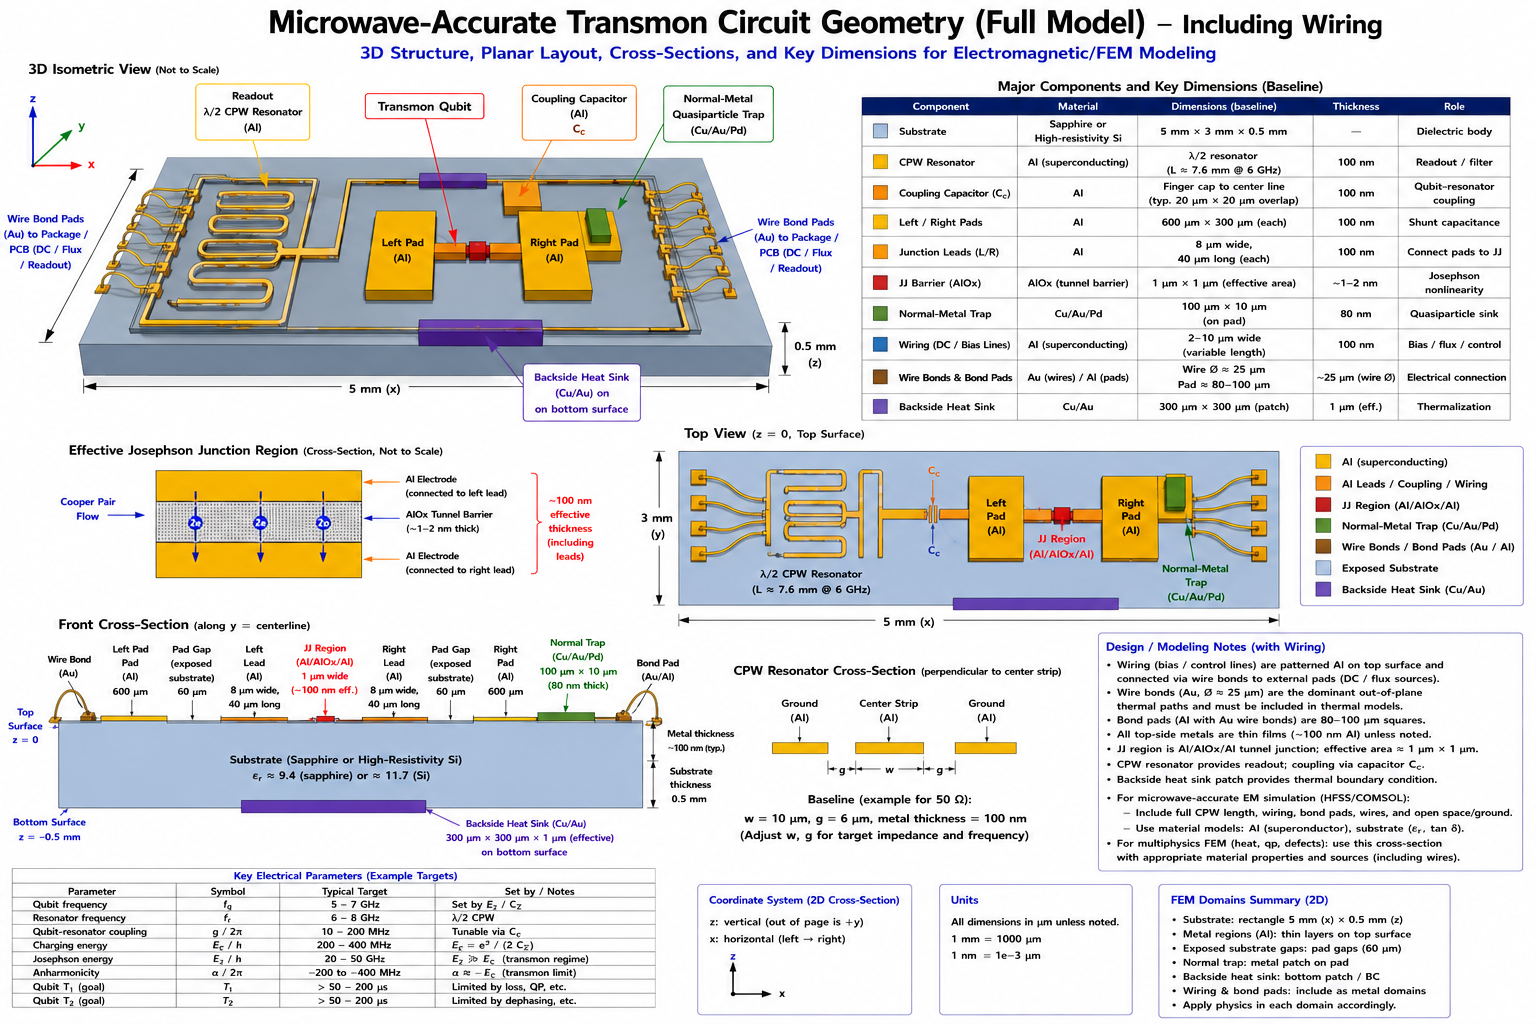
\includegraphics[width=0.97\linewidth]{figures/mod9_Transmon_RF_Wire.png}
    \caption{Full microwave-aware transmon circuit geometry with wiring. This is the physical package-level picture: a patterned superconducting microwave chip with CPW resonator, coupling capacitor, transmon pads, Josephson junction, normal-metal quasiparticle trap, backside heat sink, bond pads, and wire bonds. It is not the first MATLAB FEM domain, but it defines the physical objects that the reduced 2D model is derived from.}
    \label{fig:mod9_full_rf}
\end{figure}
\end{landscape}

\begin{landscape}
\begin{figure}[p]
    \centering
    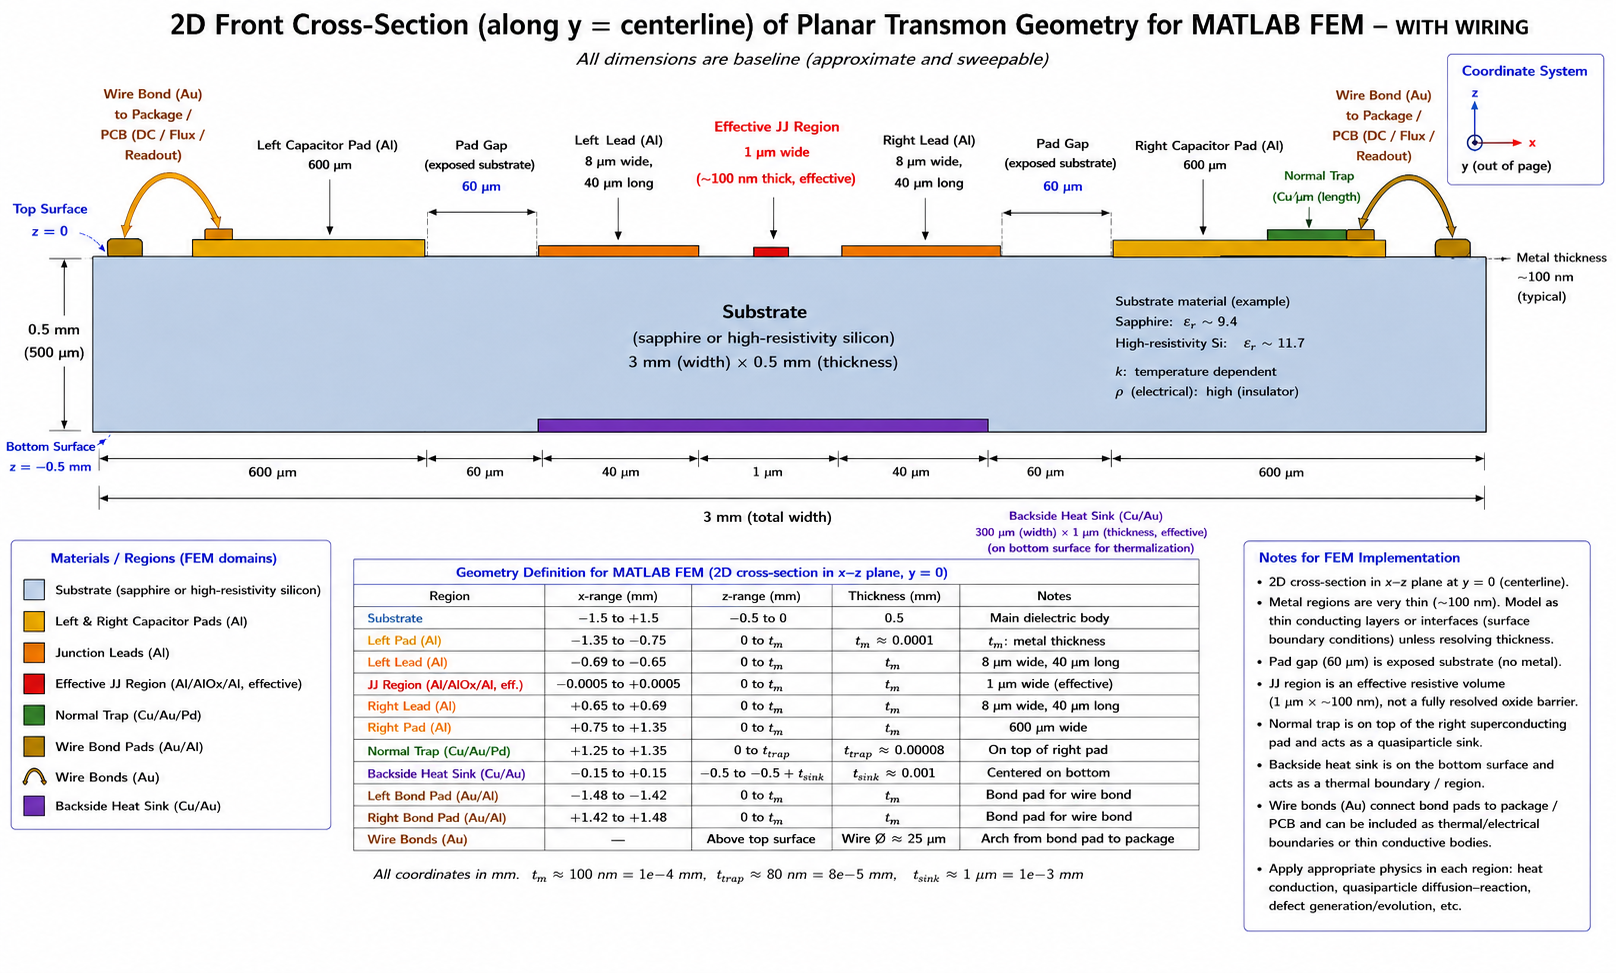
\includegraphics[width=0.97\linewidth]{figures/mod9_Transmon_2D_wire.png}
    \caption{Reduced two-dimensional front cross-section selected as the first MATLAB FEM target. The current plan is to encode all solid regions and surface/boundary patches except the curved wire-bond arcs. Wire-bond pads can be included as top metal regions; the bond-wire arcs themselves can be represented through boundary conditions or local heat/source terms applied at the bond pads.}
    \label{fig:mod9_2d_wire}
\end{figure}
\end{landscape}

\section{What physically makes this a transmon}
A planar transmon can look deceptively simple: a dielectric substrate, patterned aluminum films, and a tiny AlOx tunnel barrier. That is not a weakness of the design. The physics comes from the circuit topology and the Josephson junction, not from using many different exotic materials.

The transmon Hamiltonian, in its simplest single-junction form, is
\begin{equation}
    H = 4E_C(\hat{n}-n_g)^2 - E_J\cos\hat{\phi},
    \label{eq:transmon_hamiltonian}
\end{equation}
where
\begin{equation}
    E_C = \frac{e^2}{2C_{\Sigma}},
    \qquad
    E_J = \frac{\Phi_0 I_c}{2\pi}.
    \label{eq:EC_EJ}
\end{equation}
The large aluminum pads determine most of $C_{\Sigma}$, while the Al/AlOx/Al Josephson junction determines $E_J$ and supplies the nonlinear inductive element. The transmon regime is
\begin{equation}
    \frac{E_J}{E_C} \gg 1.
    \label{eq:transmon_regime}
\end{equation}
Increasing $C_{\Sigma}$ lowers $E_C$ and suppresses charge dispersion. The junction nonlinearity keeps the energy levels weakly anharmonic so that the lowest two levels can be used as a qubit rather than behaving as a perfectly harmonic LC oscillator.

\begin{physicsbox}
\textbf{Key physical point.} If all aluminum regions were one continuous shorted conductor, the object would not be a transmon. The two superconducting nodes are separated by an AlOx tunnel barrier. That tunnel barrier allows coherent Cooper-pair tunneling while preventing the structure from becoming an ordinary metallic short.
\end{physicsbox}

\section{Single-JJ transmon, not a SQUID baseline}
The Module 9 geometry uses one effective Josephson-junction region. Therefore the baseline is a single-JJ transmon-like device, not a DC SQUID. A DC SQUID would require two Josephson junctions in parallel around a superconducting loop:
\begin{equation}
    E_{J,\mathrm{eff}}(\Phi) \approx 2E_{J0}\cos\left(\pi\frac{\Phi}{\Phi_0}\right)
\end{equation}
for a symmetric loop. The present geometry has no loop and no second junction, so it should not be labeled a SQUID. A later Module 9 variant could replace the single JJ by a two-JJ loop if flux tunability becomes important.

\section{Detailed physical role of each region}
\subsection{Substrate}
The substrate is the mechanical, dielectric, and thermal body that supports the patterned metal. The adopted material choices are sapphire or high-resistivity silicon. Both are common because they can have low microwave loss at cryogenic temperature when prepared well, and they are compatible with planar superconducting fabrication. In this project they also provide a bridge to the original radiation-effects model, where silicon is already central.

For electromagnetic design, the substrate controls the effective dielectric constant of the CPW resonator and the capacitance between transmon pads. For thermal modeling, it is the main volume through which heat spreads from a radiation event or a dissipative wiring/bond-pad region. For defect modeling, it is the volume where radiation-induced lattice damage and trapped charge may be placed.

In the 2D MATLAB target the substrate is a rectangle,
\begin{equation}
    \Omega_{\mathrm{sub}} = \{(x,z): -1.5\,\mathrm{mm}\le x\le 1.5\,\mathrm{mm},\; -0.5\,\mathrm{mm}\le z\le 0\}.
\end{equation}
The top surface is $z=0$ and the bottom surface is $z=-0.5\,\mathrm{mm}$.

\subsection{Left and right capacitor pads}
The large aluminum capacitor pads are not arbitrary metal blocks. They are the shunt capacitance of the transmon. Their area, separation, dielectric environment, nearby ground conductors, and package geometry help determine $C_{\Sigma}$.

The electrostatic energy scale is
\begin{equation}
    E_C = \frac{e^2}{2C_{\Sigma}}.
\end{equation}
Large pads increase $C_{\Sigma}$ and reduce $E_C$. That reduction is why a transmon is much less sensitive to offset charge noise than a Cooper-pair box. In a radiation-effects model, the pads are also large superconducting reservoirs where quasiparticles can be generated, diffuse, relax, become trapped, or migrate toward the junction.

The current material is Al because aluminum is a conventional superconducting thin film with a native oxide that can form AlOx tunnel barriers. The baseline thickness is about $100\,\mathrm{nm}$, which is thin compared with the $0.5\,\mathrm{mm}$ substrate thickness.

\subsection{Pad gap and exposed substrate}
The pad gap is exposed substrate separating the two large capacitor-pad nodes. It is not a separate inserted solid. It is a region of missing metal. In the microwave circuit, this exposed substrate contributes to the capacitance between the two superconducting nodes and can host dielectric participation. Dielectric participation matters because lossy interfaces or TLS-like defects in high-field regions can degrade the qubit.

For the 2D FEM geometry, the pad-gap annotation should be interpreted as an exposed-substrate interval at the top surface. It should not break the electrical continuity of the narrow aluminum leads. The implemented lead/JJ topology must remain
\begin{equation}
    \text{left pad} \rightarrow \text{left lead} \rightarrow \Omega_{\mathrm{JJ}} \rightarrow \text{right lead} \rightarrow \text{right pad}.
\end{equation}
If an automated drawing or table suggests a disconnected lead, the connected topology overrides the drawing artifact.

\subsection{Junction leads}
The junction leads are narrow aluminum conductors that connect the capacitor pads to the junction electrodes. Their role is geometrically small but physically important. They make the circuit nodes continuous and define how quasiparticles can travel between a pad and the JJ-sensitive region.

Because the leads are narrow, they can become bottlenecks for quasiparticle diffusion and local current density. In a radiation-induced quasiparticle model, lead geometry affects the time it takes quasiparticles generated in a pad to reach the junction. In a microwave model, lead geometry also contributes parasitic inductance and capacitance.

The baseline lead width is $8\,\mu\mathrm{m}$ and the lead length is $40\,\mu\mathrm{m}$. In a 2D cross-section, the ``width'' shown along the cross-section is effectively the resolved in-plane length of the lead segment. The out-of-plane physical width is collapsed into the 2D reduction or represented by an effective thickness/area factor.

\subsection{Effective Josephson-junction region}
The real Josephson junction is an Al/AlOx/Al tunnel junction. The oxide barrier can be only about $1$--$2\,\mathrm{nm}$ thick, while the substrate is hundreds of micrometers thick. Directly meshing the barrier thickness in a full chip-scale 2D or 3D FEM model would create an extreme aspect-ratio problem.

Therefore Module 9 uses an effective JJ-sensitive region:
\begin{equation}
    \Omega_{\mathrm{JJ}} = \text{small effective volume near the physical tunnel junction}.
\end{equation}
This region is not a literal resolved oxide mesh. It is the region where radiation, heat, quasiparticle, trap, and defect exposure are scored. The baseline effective dimension is about $1\,\mu\mathrm{m}$ laterally and $100\,\mathrm{nm}$ in effective vertical thickness.

The Josephson physics is encoded by the current-phase relation
\begin{equation}
    I_s = I_c\sin\phi,
    \label{eq:josephson_current}
\end{equation}
and the voltage-phase relation
\begin{equation}
    V = \frac{\Phi_0}{2\pi}\frac{d\phi}{dt}.
    \label{eq:josephson_voltage}
\end{equation}
The nonlinearity in Eq.~\eqref{eq:josephson_current} is the source of the transmon's anharmonicity.

\subsection{Local Cooper-pair flow through the junction}
The JJ stack in the figure should be read as a local cross-section, not as a simple left-to-right metal block. The circuit path is lateral through the aluminum leads and electrodes, but the actual tunneling path is through the oxide barrier between the two superconducting electrodes. Conceptually,
\begin{equation}
    \text{left lead/electrode} \rightarrow \text{AlOx tunnel barrier} \rightarrow \text{right electrode/lead}.
\end{equation}
The local tunneling direction can be vertical through the overlap barrier, while the larger circuit connection remains left-to-right across the device.

\subsection{Normal-metal quasiparticle trap}
The normal trap is a Cu/Au/Pd region placed on or near a superconducting pad. Its purpose is to remove quasiparticles from the superconducting aluminum before they diffuse to the JJ. In a reduced diffusion-reaction equation, the trap contributes a local sink term,
\begin{equation}
    \frac{\partial n_{\mathrm{qp}}}{\partial t}
    = \nabla\cdot(D_{\mathrm{qp}}\nabla n_{\mathrm{qp}})
    - \Gamma_{\mathrm{trap}}(\mathbf{r}) n_{\mathrm{qp}}
    - \Gamma_{\mathrm{rec}} n_{\mathrm{qp}}
    + S_{\mathrm{qp}}(\mathbf{r},t).
    \label{eq:qp_trap_model}
\end{equation}
The trap must be physically coupled to the superconducting metal. If it were placed only on bare substrate with no superconducting contact or tunneling/proximity coupling, it would not efficiently drain quasiparticles from the Al film. It might still act as a phonon or thermal absorber, but that is a different function.

The baseline placement is on the right capacitor pad, away from the JJ. This placement is physically sensible because it gives quasiparticles a sink without directly contaminating the JJ region or bridging the two transmon nodes. The normal trap should not short the two capacitor pads.

\subsection{Backside heat sink}
The backside heat sink is a bottom-surface thermalization region, not a top-side quasiparticle trap. Its purpose is to represent coupling to a cold stage, package ground, backside metallization, or thermal anchor. The baseline material is Cu/Au and the baseline patch size is about $300\,\mu\mathrm{m}\times300\,\mu\mathrm{m}$ with $1\,\mu\mathrm{m}$ effective thickness if meshed.

In the first MATLAB FEM thermal implementation, the heat sink can be represented more cleanly as a boundary condition on the bottom surface:
\begin{equation}
    -k\nabla T\cdot\mathbf{n} = h_{\mathrm{sink}}(T-T_0)
    \qquad \text{on } \Gamma_{\mathrm{sink}},
    \label{eq:robin_sink}
\end{equation}
where $h_{\mathrm{sink}}$ is an effective thermal boundary conductance. A stronger idealization is a Dirichlet cold patch,
\begin{equation}
    T=T_0 \qquad \text{on } \Gamma_{\mathrm{sink}}.
    \label{eq:dirichlet_sink}
\end{equation}
The Robin form is usually more physical because real thermalization is finite.

\subsection{CPW resonator and feedline structures}
The full microwave-aware geometry contains a CPW resonator. A CPW consists of a center strip and two neighboring ground conductors patterned on the same surface. It supports microwave modes whose fields extend into the substrate and surrounding vacuum. The resonator is used for readout and can also mediate coupling between an external microwave line and the transmon.

For a rough half-wave resonator,
\begin{equation}
    L \approx \frac{v_p}{2 f_r},
\end{equation}
where $v_p\approx c/\sqrt{\epsilon_{\mathrm{eff}}}$ is the phase velocity and $f_r$ is the resonator frequency. A few-GHz resonator on a dielectric substrate therefore naturally has a millimeter-scale electrical length. In the full drawing, the resonator is meandered so that this length fits on the chip.

The CPW is not part of the first 2D transmon-centerline FEM geometry unless the chosen cross-section explicitly cuts through it. For microwave-accurate simulations, however, the CPW, ground planes, coupling capacitor, chip edges, wire bonds, package walls, and launch geometry all matter.

\subsection{Coupling capacitor}
The coupling capacitor $C_c$ connects the resonator/feedline electromagnetic mode to the transmon without creating a DC short. It sets the qubit-resonator coupling strength and readout access. In a circuit model, the relevant parameter is often the coupling rate $g$ or a dispersive shift $\chi$ derived from the qubit-resonator coupling.

For thermal and radiation modeling, the coupling capacitor is also a patterned metal region where local fields and losses can occur. In the first 2D front cross-section, it is not included unless the section is chosen through the coupling feature. In a later full-chip EM/FEM model it should be represented.

\subsection{Bond pads, wire bonds, and wiring}
Wire bonds connect on-chip bond pads to package traces, PCBs, coaxial launches, ground, flux-bias lines, DC lines, or microwave readout/control lines. They carry AC microwave currents, DC or low-frequency currents if a bias line is present, and heat conducted from the package environment. They are therefore both electrical and thermal boundary features.

The wire bond is not a DC power cable for the transmon island. In superconducting qubit operation, the device is controlled and read out by microwave electromagnetic fields. The physical path is approximately
\begin{equation}
\begin{aligned}
&\text{room-temperature source}
\rightarrow \text{coaxial line}
\rightarrow \text{attenuators/filters} \\
&\rightarrow \text{package launch}
\rightarrow \text{wire bond}
\rightarrow \text{on-chip CPW/feedline/control line}.
\end{aligned}
\label{eq:wire_signal_path}
\end{equation}
At the chip, the microwave field couples to a resonator, feedline, drive line, or flux line. Equation~\eqref{eq:wire_signal_path} is deliberately split across two lines so the signal path remains visible in the PDF and does not run past the page margin.

For Module 9 thermal modeling, the important effect is that wiring can add a local heat source or a thermal link. Possible terms include
\begin{equation}
    Q_{\mathrm{wire}}(\mathbf{r},t),
    \label{eq:qwire}
\end{equation}
for local dissipative heating, or a boundary flux
\begin{equation}
    -k\nabla T\cdot\mathbf{n} = q_{\mathrm{wire}}(x,t)
    \qquad \text{on } \Gamma_{\mathrm{wire}}.
    \label{eq:wire_flux}
\end{equation}
The wire-bond arc itself is above the substrate. In the first 2D MATLAB model, do not mesh the arc. Instead, mesh or tag the bond pad and apply a source, flux, or thermal-link condition there if wiring heating is being studied.

\section{Material choices and solid-state physics rationale}
The material choices in Module 9 are not arbitrary labels for drawing regions. Each material is selected because its electronic structure, bonding chemistry, superconducting behavior, microwave loss, thermal transport, and fabrication compatibility support a specific role in the transmon package. A useful way to read the geometry is therefore not as ``many rectangles,'' but as a deliberately arranged solid-state system:
\begin{equation}
\begin{aligned}
\text{Module 9 material stack}
&= \text{dielectric substrate}
 + \text{superconducting Al circuit} \\
&\quad + \text{AlOx tunnel barrier}
 + \text{normal-metal relaxation paths} \\
&\quad + \text{package thermalization paths}.
\end{aligned}
\end{equation}
The first MATLAB model does not need atomistic material physics, but it does need material-aware coefficients. In later modules these choices determine dielectric permittivity, loss tangent, heat capacity, thermal conductivity, quasiparticle diffusivity, quasiparticle recombination/trapping rates, carrier mobility, defect-generation rates, and boundary thermal conductance.

\subsection{Periodic-table view of the baseline material set}
The baseline transmon package uses a small set of elements with very different electronic roles:
\begin{itemize}[leftmargin=1.5em]
    \item \textbf{Aluminum, Al, atomic number 13}: a group-13 simple metal with three valence electrons. In the thin films of the qubit circuit it is a superconductor at dilution-refrigerator temperature and forms the native oxide used as the Josephson tunnel barrier.
    \item \textbf{Silicon, Si, atomic number 14}: a group-14 covalent semiconductor with diamond-cubic bonding. In high-resistivity form it behaves as a low-loss dielectric/mechanical substrate rather than as an ordinary conducting semiconductor.
    \item \textbf{Sapphire, $\mathrm{Al_2O_3}$}: a crystalline ionic/covalent oxide composed of Al and O. It is not a metal; it is a wide-band-gap insulating substrate with good microwave and cryogenic properties when high purity and well prepared.
    \item \textbf{Oxygen, O, atomic number 8}: not used as a metal region, but chemically central because oxygen turns aluminum into aluminum oxide, $\mathrm{AlO_x}$ or approximately $\mathrm{Al_2O_3}$, which is the tunnel barrier.
    \item \textbf{Copper, Cu, atomic number 29}: a group-11 normal metal with high electrical and thermal conductivity. It is useful for thermalization and quasiparticle trapping because it remains a normal metallic reservoir at the temperatures of interest.
    \item \textbf{Gold, Au, atomic number 79}: a noble group-11 metal with excellent chemical stability, high conductivity, and good wire-bond/package compatibility. Its chemical inertness is valuable because uncontrolled oxides and surface chemistry can create microwave loss and poor contacts.
    \item \textbf{Palladium, Pd, atomic number 46}: a transition metal with a large density of electronic states near the Fermi level and useful contact/proximity behavior in normal-metal trap stacks.
\end{itemize}
The geometry therefore combines three material classes: superconductors, insulators/dielectrics, and normal metals. The transmon needs all three. The superconductor supplies a coherent condensate and low microwave loss; the insulator supplies capacitance and the tunnel barrier; the normal metals supply dissipative relaxation and thermalization channels that the superconducting condensate itself cannot efficiently provide.

\subsection{Substrate: sapphire or high-resistivity silicon}
The substrate is the largest volume in the geometry. It supports the metal pattern mechanically, sets much of the microwave dielectric environment, stores and transports phonons, and receives a large fraction of the radiation-induced energy deposition in many scenarios.

\subsubsection{Why an insulating or high-resistivity substrate is needed}
A transmon should not sit on a lossy conducting slab. If the substrate had significant microwave conductivity, the resonator and qubit fields would drive currents in the substrate, converting microwave energy into heat. That loss would lower resonator quality factor and qubit coherence. Therefore the substrate must act primarily as a dielectric at the qubit frequency. In an electromagnetic model, the substrate enters through
\begin{equation}
    \mathbf{D}=\epsilon \mathbf{E},
    \qquad
    P_{\mathrm{diel}} \propto \omega \epsilon'' |\mathbf{E}|^2,
\end{equation}
where $\epsilon''$ is the lossy part of the dielectric response. The engineering objective is small dielectric loss in the regions where the microwave electric field is large, especially pad gaps, substrate surfaces, and metal-substrate interfaces.

\subsubsection{Sapphire as a substrate}
Sapphire is crystalline $\mathrm{Al_2O_3}$. From a bonding perspective it is an oxide: aluminum atoms are electropositive relative to oxygen, and the resulting solid has a large band gap and no free-electron sea. This makes sapphire a dielectric rather than a metal. Its useful properties for superconducting microwave circuits are:
\begin{itemize}[leftmargin=1.5em]
    \item \textbf{Low free-carrier density.} With no intentional carriers, sapphire does not provide an easy ohmic path for microwave dissipation.
    \item \textbf{Good crystalline order.} A high-quality crystal has fewer bulk disorder sites than an amorphous dielectric, reducing one source of TLS-like loss.
    \item \textbf{Mechanical and thermal stability.} It is a rigid substrate that can support thin films and survive processing.
    \item \textbf{Dielectric participation control.} Its dielectric constant and geometry shape the CPW resonator velocity, transmon capacitance, and electric-field participation.
\end{itemize}
The weakness of sapphire for this project is that it is not the original silicon radiation-effects substrate. A sapphire model is excellent for transmon relevance, but high-resistivity silicon gives a more direct bridge to the earlier defect, carrier, and electrostatic modules.

\subsubsection{High-resistivity silicon as a substrate}
Silicon is a group-IV covalent semiconductor. Each Si atom forms four tetrahedral bonds in the diamond-cubic lattice. In ordinary electronics, silicon is useful because doping can tune its carrier density. For a qubit substrate, the opposite is desired: high resistivity, low carrier density, and low microwave loss. High-resistivity silicon is therefore treated as a dielectric-like body at low temperature, not as a conducting device channel.

Silicon is especially useful for RadiationEffects\_proj2 because the existing project already models silicon radiation damage. Radiation can create electron-hole pairs, lattice defects, trapped charge, and local phonons. Thus high-resistivity Si lets Module 9 inherit the earlier language of defect concentrations $c_j$, carrier densities $n,p$, electrostatic fields $\varphi$, and recombination/trapping terms. The penalty is that Si surfaces, native oxide, impurity residues, and interface states can contribute to charge noise and microwave loss if not controlled.

\subsubsection{Substrate role in the FEM model}
For MATLAB FEM, the substrate should be the main 2D or 3D domain. It receives material parameters such as
\begin{equation}
    \epsilon_r,\quad k(T),\quad C(T),\quad \rho_{\mathrm{mass}},\quad D_j(T),\quad \mu_n(T),\quad \mu_p(T),
\end{equation}
with the understanding that not every module uses every coefficient. In the prompt qubit-error problem, substrate phonons and trapped charge are often more important than slow thermally activated lattice-defect diffusion at millikelvin temperature. In long-term accumulated-damage studies, defect populations and trapped charge become more important.

\subsection{Aluminum for capacitor pads, junction leads, CPW, and JJ electrodes}
Aluminum is the central superconducting material in the baseline geometry. It is used for the large capacitor pads, narrow junction leads, CPW resonator, coupling structures, and the two JJ electrodes.

\subsubsection{Al as a simple metal}
Aluminum is a light group-13 metal with three valence electrons. In a normal-metal picture, these valence electrons form broad conduction bands and a Fermi sea. This makes Al easy to use as a low-resistance thin-film conductor before considering superconductivity. It can be evaporated or sputtered, patterned by liftoff or etching, and integrated with standard planar microfabrication.

\subsubsection{Al as a superconductor}
At dilution-refrigerator temperatures aluminum is superconducting. The key microscopic fact is that below its superconducting transition temperature $T_c$ the electrons near the Fermi surface form Cooper pairs. In BCS language, the excitation spectrum develops an energy gap $\Delta$:
\begin{equation}
    E_k = \sqrt{\xi_k^2+\Delta^2}.
\end{equation}
The gap matters because a phonon or other excitation with energy greater than approximately $2\Delta$ can break a Cooper pair and generate quasiparticles. For aluminum, typical values are
\begin{equation}
    T_c \approx 1.2\,\mathrm{K},
    \qquad
    \Delta_{\mathrm{Al}} \sim 180\text{--}200\,\mu\mathrm{eV},
    \qquad
    2\Delta_{\mathrm{Al}} \sim 360\text{--}400\,\mu\mathrm{eV}.
\end{equation}
This is good for making a superconducting microwave circuit at $10$--$30\,\mathrm{mK}$, but it also creates a radiation vulnerability: pair-breaking phonons can populate the Al films with quasiparticles.

\subsubsection{Why Al is used for pads and leads}
The capacitor pads must be superconducting conductors with low microwave loss. Their large area creates the shunt capacitance $C_{\Sigma}$, which lowers
\begin{equation}
    E_C=\frac{e^2}{2C_{\Sigma}}.
\end{equation}
The narrow leads must be continuous with the pads and JJ electrodes. They define the geometric bottleneck between the large quasiparticle reservoirs and the JJ-sensitive region. Using the same Al film for pads and leads gives clean superconducting continuity and avoids extra interfaces that could add microwave loss, contact resistance, or uncontrolled proximity effects.

\subsubsection{Why Al is used for the Josephson-junction electrodes}
The strongest practical reason for Al is not merely that it superconducts. It is that aluminum forms a controllable native oxide. A standard tunnel junction can be fabricated as
\begin{equation}
    \mathrm{Al}\,/\,\mathrm{AlO_x}\,/\,\mathrm{Al}.
\end{equation}
The oxide thickness and oxidation conditions control the normal-state tunnel resistance, which controls the critical current $I_c$ and therefore
\begin{equation}
    E_J=\frac{\Phi_0 I_c}{2\pi}.
\end{equation}
This material stack gives the nonlinear Josephson current-phase relation
\begin{equation}
    I_s=I_c\sin\phi.
\end{equation}
Without the AlOx barrier, the left and right superconducting nodes would be directly shorted and the transmon would lose its nonlinear element.

\subsubsection{Al is not chosen primarily as a heat sink}
Aluminum is not thermally ideal in the superconducting state. Once Al becomes superconducting, the electronic heat capacity and normal electronic thermal conductivity are strongly suppressed at low temperature because most electrons are in the condensate. Heat can still move through phonons and quasiparticles, but the superconducting film is not a robust dissipative thermal dump. This is why Module 9 includes normal-metal traps and backside thermal sinks. In model language,
\begin{equation}
\begin{aligned}
\text{Al regions} &\rightarrow \text{low-loss superconducting circuit}, \\
\text{Cu/Au/Pd regions} &\rightarrow \text{relaxation and thermalization channels}.
\end{aligned}
\end{equation}

\subsection{Aluminum oxide tunnel barrier: small chemically, dominant physically}
The AlOx barrier is geometrically tiny but physically decisive. Chemically it is an aluminum-oxygen compound, approximately related to $\mathrm{Al_2O_3}$ but often written $\mathrm{AlO_x}$ because real tunnel barriers can be nonstoichiometric and disordered. Electronically it is an insulator. Its role is to block ordinary metallic conduction while allowing quantum tunneling of Cooper pairs.

A useful solid-state picture is a barrier of height $U_0$ and thickness $d$. The tunneling amplitude depends approximately exponentially on barrier thickness,
\begin{equation}
    \mathcal{T} \sim \exp(-2\kappa d),
    \qquad
    \kappa \approx \frac{\sqrt{2m(U_0-E)}}{\hbar}.
\end{equation}
That exponential sensitivity is why oxidation control is so important. A change of only an atomic-scale thickness can noticeably change $I_c$ and $E_J$. The barrier also introduces a materials problem: amorphous or defective oxides can host TLSs. Those TLSs can couple to microwave electric fields in the junction or nearby surfaces and produce loss or noise. Thus AlOx is simultaneously the enabling element of the Josephson junction and one of the most sensitive material regions.

For Module 9 FEM, the oxide is not meshed explicitly in the first implementation. Instead, $\Omega_{\mathrm{JJ}}$ is an effective region where radiation, quasiparticle, thermal, charge, and defect exposure are scored.

\subsection{Normal-metal quasiparticle trap: Cu/Au/Pd}
The normal-metal trap is deliberately not superconducting. Its purpose is to provide a place where quasiparticles in the Al film can relax before reaching the Josephson junction. In a reduced model this appears as a local sink term,
\begin{equation}
    -\Gamma_{\mathrm{trap}}(\mathbf{r})n_{\mathrm{qp}}.
\end{equation}
The trap only works as a quasiparticle trap if it is electrically or proximity-coupled to the superconducting metal. A normal-metal rectangle floating on bare substrate is not an efficient Al quasiparticle drain; it is at most a phonon or thermal absorber.

\subsubsection{Why copper helps}
Copper is a highly conductive normal metal with mobile electrons at the Fermi level. It does not become superconducting in the ordinary operating range relevant here, so it retains a continuous quasiparticle density of states at low energy. When a quasiparticle reaches a Cu-coupled trap, it can enter or relax into normal-metal electronic states rather than remaining in the superconducting Al excitation spectrum. Copper is also a strong thermal conductor, which helps spread and remove dissipated energy if it is well thermalized.

In the FEM model, Cu-like behavior motivates large electronic/thermal diffusivity and a trap coefficient $\Gamma_{\mathrm{trap}}$ in the trap region or at the trap-pad interface. The exact value is not determined by the element name alone; it depends on interface transparency, oxide thickness, trap geometry, disorder, and temperature.

\subsubsection{Why gold helps}
Gold is chemically noble. It resists forming a thick native insulating oxide under ordinary processing conditions. That matters because uncontrolled oxides at metal interfaces can block electrical/thermal contact, create TLS-like defects, and make properties drift. Gold is also ductile and bondable, which is why it is common in wire bonds, pads, and package metallization. Its high atomic number and strong electron system make it useful as a robust normal-metal thermalization layer.

Gold's advantage is therefore not that it is superconducting; it is useful precisely as a stable normal metal. In a trap or backside metallization stack, Au can protect surfaces, improve contact to package structures, and provide a chemically stable conducting layer. The caution is that any normal metal placed in a high microwave-field region can add loss if it is not placed carefully.

\subsubsection{Why palladium may be used}
Palladium is a transition metal with a large density of electronic states near the Fermi level. It is often used in multilayer normal-metal structures because it can provide good contact/proximity behavior with superconducting films and can help tailor quasiparticle relaxation. In simplified Module 9 language, Pd represents a normal-metal layer that can improve the trap's ability to absorb excitations from the Al without becoming a superconducting short across the qubit nodes.

The exact stack Cu/Au/Pd should not be interpreted as a universal recipe. It is a placeholder for a normal-metal trap family. The model should allow the user to change $\Gamma_{\mathrm{trap}}$, trap geometry, and interface transparency independently.

\subsubsection{Why the trap is placed on one pad and away from the JJ}
The trap is placed on a superconducting pad because that is where it can couple to the Al quasiparticle population. It is placed away from the JJ because the JJ is the most microwave- and coherence-sensitive region. A normal metal close to the junction could introduce excess loss, alter the local electromagnetic environment, or create uncontrolled proximity effects. The trap must also not bridge the left and right pads; otherwise it would create a dissipative shunt across the qubit nodes.

Thus the design rule is
\begin{equation}
    \text{strong enough coupling to drain quasiparticles}
    \quad + \quad
    \text{far enough from the JJ to avoid added loss}.
\end{equation}
This tradeoff is one of the natural geometry sweeps for RadiationEffects\_proj2.

\subsection{Backside heat sink: Cu/Au thermalization patch}
The backside heat sink is a thermalization feature on the bottom surface of the substrate. It should not be interpreted as a top-side normal trap. Its function is to remove substrate heat and provide a simplified representation of the chip-to-package thermal path.

\subsubsection{Why copper and gold are natural backside metals}
Copper and gold are normal metals with high thermal conductivity at low temperature when clean and well connected. The relevant solid-state mechanism is the mobile electron gas: in a normal metal, electrons carry both charge and heat. At low temperature, the relation between electrical and electronic thermal conductivity is often organized by the Wiedemann-Franz idea,
\begin{equation}
    \frac{k_e}{\sigma T} \approx L_0,
\end{equation}
where $L_0$ is the Lorenz number, $\sigma$ is electrical conductivity, and $k_e$ is electronic thermal conductivity. This is not a full cryogenic package model, but it explains why good normal metals are attractive thermal links.

Copper is usually valued for high thermal conductivity. Gold is valued for chemical stability, contact reliability, and compatibility with bonding/metallization. In a multilayer thermalization patch, Cu may provide strong thermal conduction while Au may provide a stable surface and reliable contact.

\subsubsection{How the backside sink enters the FEM model}
The first FEM model should usually treat the backside sink as a boundary condition rather than a fully resolved $1\,\mu\mathrm{m}$ layer. A Robin condition,
\begin{equation}
    -k\nabla T\cdot\mathbf{n}=h_{\mathrm{sink}}(T-T_0),
\end{equation}
is more realistic than an ideal fixed-temperature patch because real die attach, interface roughness, acoustic mismatch, Kapitza boundary resistance, and package geometry all limit heat transfer. A Dirichlet condition $T=T_0$ is useful as a strong-sink limit.

The backside sink can also represent phonon removal or phonon downconversion in a coarse model. Radiation events in the substrate can generate high-energy phonons. A bottom thermalization patch gives those phonons or their thermalized descendants a path out of the substrate, reducing energy available to generate quasiparticles in the top Al films.

\subsection{Bond pads and wire bonds: Al/Au package interfaces}
Bond pads and wire bonds are package-interface materials, not qubit-island power supplies. The transmon is driven and read out by microwave electromagnetic fields. The wires and package traces deliver AC signals, DC/low-frequency bias if present, ground connections, and thermal links.

\subsubsection{Al bond pads}
Al bond pads are natural when the on-chip wiring and CPW metal are patterned in the same Al layer. This avoids adding unnecessary metal interfaces and preserves process simplicity. In an FEM thermal model, a bond pad is a localized metal patch where heat can enter from package wiring or be removed to a thermalized package ground.

\subsubsection{Au wire bonds}
Gold wire is widely used because it is ductile, chemically stable, and bondable. The wire bond is not included as a meshed curved domain in the first 2D model because it lies above the substrate surface and belongs to the package domain. Its effect should enter through the bond pad as
\begin{equation}
    P_{\mathrm{wire}} = G_{\mathrm{wire}}(T_{\mathrm{pkg}}-T_{\mathrm{pad}})+P_{\mathrm{diss}}(t).
\end{equation}
The same physical wire can be a microwave conductor, a thermal conductor, and a source of parasitic inductance. For microwave accuracy, wire-bond inductance and package geometry matter. For the first RadiationEffects\_proj2 transport model, the most important effect is localized heat or thermal leakage at the bond pads.

\subsection{CPW resonator and coupling capacitor materials}
The CPW resonator and coupling capacitor are drawn in the full microwave-aware figure but are mostly outside the centerline 2D transport target. They are still important for understanding the physical device.

The CPW resonator uses superconducting Al because microwave currents should flow with minimal ohmic loss. The resonance frequency is not set by Al alone; it is set by geometry and dielectric environment:
\begin{equation}
    f_r \sim \frac{v_p}{2L},
    \qquad
    v_p\approx \frac{c}{\sqrt{\epsilon_{\mathrm{eff}}}}.
\end{equation}
The coupling capacitor is also Al because it is a patterned superconducting conductor. Its function is geometric and electromagnetic: it permits capacitive microwave coupling while avoiding a DC short. For Module 9, the important lesson is that the microwave structure should be superconducting and low loss, but the thermal and quasiparticle mitigation structures are often normal-metal regions placed carefully away from high-field regions.

\subsection{Material roles summarized for implementation}
\begin{longtable}{>{\RaggedRight\arraybackslash}p{0.15\linewidth} >{\RaggedRight\arraybackslash}p{0.15\linewidth} >{\RaggedRight\arraybackslash}p{0.31\linewidth} >{\RaggedRight\arraybackslash}p{0.29\linewidth}}
\toprule
\textbf{Region} & \textbf{Baseline material} & \textbf{Solid-state reason} & \textbf{Modeling implication}\\
\midrule
Substrate & Sapphire or high-resistivity Si & Low free-carrier density, dielectric behavior, mechanical support, phonon host. & Main domain for heat, phonons, charge trapping, defects, and electrostatics.\\
Pads, leads, CPW & Al & Superconducting thin film, low microwave loss, mature fabrication. & Superconducting domains; QP generation/diffusion regions; thin-film or surface regions.\\
JJ barrier & AlOx & Insulating tunnel barrier formed by controlled oxidation of Al. & Do not mesh atomistically initially; use effective JJ scoring domain.\\
Normal trap & Cu/Au/Pd & Normal-metal density of states and relaxation; chemical/contact stability. & QP sink term or trap boundary/interface on one pad.\\
Backside sink & Cu/Au & High-conductivity normal-metal thermalization path to package/cold stage. & Bottom Robin/Dirichlet thermal boundary or thin sink patch.\\
Bond pads/wires & Al/Au & Process-compatible pads and ductile, stable, conductive package wires. & Bond pads are top regions; wire arcs become boundary/source terms.\\
\bottomrule
\end{longtable}

\begin{notebox}
\textbf{Modeling caution.} Material names alone do not determine all coefficients. The quasiparticle trap rate, microwave loss, thermal boundary conductance, and defect/trap density are dominated by interfaces, disorder, oxidation, fabrication history, and geometry. Module 9 should therefore treat material choice as a physically informed starting point, while leaving coefficients sweepable.
\end{notebox}

\section{Code-ready 2D geometry convention}
The final image is a schematic. For the MATLAB geometry builder, the most important requirement is topological correctness. The code geometry should enforce continuous metal connectivity between pads, leads, and the effective JJ region. The following coordinate convention is recommended for the first MATLAB implementation.

\subsection{Coordinate system}
Use the 2D cross-section plane
\begin{equation}
    (x,z) \in [-1.5,1.5]\,\mathrm{mm}\times[-0.5,0]\,\mathrm{mm},
\end{equation}
with $z=0$ at the top surface and $z=-0.5\,\mathrm{mm}$ at the bottom surface. The out-of-plane coordinate $y$ is collapsed.

Let
\begin{equation}
    t_m=10^{-4}\,\mathrm{mm},\qquad
    t_{\mathrm{trap}}=8\times10^{-5}\,\mathrm{mm},\qquad
    t_{\mathrm{sink}}=10^{-3}\,\mathrm{mm}.
\end{equation}
These thicknesses are much smaller than the substrate thickness. The first solver can either resolve them using thin elements or treat them as surface/interface regions with effective conductance/source terms.

\subsection{Connected central transmon geometry}
The following central geometry preserves the requested baseline values while keeping connectivity:
\begin{itemize}[leftmargin=1.5em]
    \item pad gap between large pad inner edges: $60\,\mu\mathrm{m}$;
    \item left pad inner edge: $x=-0.030\,\mathrm{mm}$;
    \item right pad inner edge: $x=+0.030\,\mathrm{mm}$;
    \item effective JJ region: $x\in[-0.0005,+0.0005]$ mm;
    \item left lead: $x\in[-0.0405,-0.0005]$ mm, so it touches the JJ and overlaps the left pad slightly;
    \item right lead: $x\in[+0.0005,+0.0405]$ mm, so it touches the JJ and overlaps the right pad slightly;
    \item left pad: $x\in[-0.630,-0.030]$ mm;
    \item right pad: $x\in[+0.030,+0.630]$ mm.
\end{itemize}
The small lead-pad overlap is intentional. It prevents a numerical gap between the pad and the lead while preserving the $60\,\mu\mathrm{m}$ exposed pad-gap dimension between large pad edges.

\begin{notebox}
\textbf{Important correction for implementation.} The generated illustration is a visual target, but any inconsistent numeric table produced by an image generator should not be copied blindly. The MATLAB geometry must be connected: left pad touches left lead, left lead touches the JJ region, the JJ region touches the right lead, and the right lead touches the right pad.
\end{notebox}

\subsection{Recommended 2D region table}
\begin{longtable}{>{\RaggedRight\arraybackslash}p{0.21\linewidth} >{\RaggedRight\arraybackslash}p{0.22\linewidth} >{\RaggedRight\arraybackslash}p{0.22\linewidth} >{\RaggedRight\arraybackslash}p{0.25\linewidth}}
\toprule
\textbf{Region} & \textbf{$x$ range (mm)} & \textbf{$z$ range (mm)} & \textbf{Implementation meaning}\\
\midrule
Substrate & $[-1.5,+1.5]$ & $[-0.5,0]$ & Main dielectric/semiconductor body.\\
Left capacitor pad & $[-0.630,-0.030]$ & $[0,t_m]$ & Superconducting left node; shunt capacitance and QP reservoir.\\
Right capacitor pad & $[+0.030,+0.630]$ & $[0,t_m]$ & Superconducting right node; shunt capacitance and QP reservoir.\\
Pad gap & $[-0.030,+0.030]$ except where lead/JJ metal is present & top exposed surface & Exposed substrate gap; not a separate material and not a disconnected block.\\
Left junction lead & $[-0.0405,-0.0005]$ & $[0,t_m]$ & Al lead connecting left pad to JJ; overlaps left pad over $10.5\,\mu\mathrm{m}$.\\
Effective JJ region & $[-0.0005,+0.0005]$ & $[0,t_m]$ & Effective JJ-sensitive scoring region; not a fully resolved oxide mesh.\\
Right junction lead & $[+0.0005,+0.0405]$ & $[0,t_m]$ & Al lead connecting JJ to right pad; overlaps right pad over $10.5\,\mu\mathrm{m}$.\\
Normal-metal trap & e.g. $[+0.450,+0.550]$ & $[t_m,t_m+t_{\mathrm{trap}}]$ & Cu/Au/Pd trap on top of the right pad; can also be represented as a tagged surface sink on the right pad.\\
Backside heat-sink patch & $[-0.150,+0.150]$ & $[-0.5,-0.5+t_{\mathrm{sink}}]$ or boundary only & Cu/Au bottom thermal patch or Robin/Dirichlet thermal boundary on $z=-0.5\,\mathrm{mm}$.\\
Left bond pad & e.g. $[-1.48,-1.40]$ & $[0,t_m]$ & On-chip bond pad for package/wiring boundary condition.\\
Right bond pad & e.g. $[+1.40,+1.48]$ & $[0,t_m]$ & On-chip bond pad for package/wiring boundary condition.\\
Wire-bond arc & not meshed in first 2D model & above $z=0$ & Represent by boundary flux/source/thermal link at bond pad if needed.\\
\bottomrule
\end{longtable}

\section{How Module 9 connects to existing modules}
\subsection{Module 1: radiation source mapping}
Module 1 supplies deposited energy. In the transmon geometry the source can be placed in the substrate, metal films, trap, heat sink, or near the JJ-sensitive region. A deposited-energy density $E_{\mathrm{dep}}(x,z)$ can be converted into a heat source
\begin{equation}
    Q_{\mathrm{rad}}(x,z,t) = \frac{E_{\mathrm{dep}}(x,z)}{\Delta t}
\end{equation}
or a defect-generation source
\begin{equation}
    G_d(x,z,t)=\eta_d \frac{Q_{\mathrm{rad}}(x,z,t)}{E_{d,\mathrm{form}}},
\end{equation}
where $\eta_d$ is an efficiency factor and $E_{d,\mathrm{form}}$ is an effective defect-formation energy scale.

\subsection{Module 2: electrostatics and offset charge}
In the superconducting transmon case, Module 2 can serve two roles. First, it can solve the electrostatic field in the substrate and gap regions due to trapped charge or radiation-induced charge. Second, it can estimate how trapped charge near high-field regions affects offset charge, surface participation, and local field stress. The full microwave capacitance matrix is not yet solved by the MATLAB 2D FEM scaffold, but the Module 9 geometry gives the spatial regions where such a later EM solve would be performed.

The basic electrostatic equation is
\begin{equation}
    -\nabla\cdot(\epsilon\nabla\varphi)=\rho_{\mathrm{trap}}+\rho_{\mathrm{defect}}+\rho_{\mathrm{bias}}.
\end{equation}
For a full microwave-accurate model, the same geometry would be used in an eigenmode or driven-frequency EM solve rather than only a DC/low-frequency Poisson solve.

\subsection{Module 3: defects and traps}
Defect evolution in the substrate can still be represented by diffusion-reaction equations,
\begin{equation}
    \frac{\partial c_j}{\partial t}=\nabla\cdot(D_j\nabla c_j)+G_j-R_j,
\end{equation}
with material-dependent coefficients. In the superconducting geometry, special attention should be given to defects near surfaces, metal-substrate interfaces, pad-gap regions, and the JJ-sensitive region because they can act as TLSs, charge traps, or recombination centers.

\subsection{Module 4: thermal transport}
Module 4 becomes especially important because radiation, wiring, and microwave dissipation can create local heating. A baseline thermal equation is
\begin{equation}
    C(\mathbf{r})\frac{\partial T}{\partial t}=\nabla\cdot(k(\mathbf{r})\nabla T)+Q_{\mathrm{rad}}+Q_{\mathrm{wire}}+Q_{\mathrm{mw}}.
\end{equation}
The backside sink appears as a bottom boundary condition or thin thermal region. Bond pads can appear as localized heating or thermal leakage points.

\subsection{Module 5: quasiparticle and carrier response}
For a superconducting transmon, the most relevant mobile excitation may be quasiparticles rather than ordinary semiconductor electrons and holes. A reduced quasiparticle equation is
\begin{equation}
    \frac{\partial n_{\mathrm{qp}}}{\partial t}
    = \nabla\cdot(D_{\mathrm{qp}}\nabla n_{\mathrm{qp}})
    - \Gamma_{\mathrm{rec}}n_{\mathrm{qp}}
    - \Gamma_{\mathrm{trap}}(\mathbf{r})n_{\mathrm{qp}}
    + S_{\mathrm{qp}}(\mathbf{r},t).
\end{equation}
Here $S_{\mathrm{qp}}$ can be driven by pair-breaking phonons, radiation-induced energy deposition, or local microwave/thermal injection. The trap term is nonzero in $\Omega_{\mathrm{trap}}$ or at the trap-pad interface.

\subsection{Module 6: coupled superconducting multiphysics}
Module 6 can use Module 9 as a tagged geometry. The coupled state may include
\begin{equation}
    \mathbf{u}=\{T, c_j, \varphi, n_{\mathrm{qp}}, q_{\mathrm{trap}}, J_{\mathrm{JJ}}\}.
\end{equation}
The module then connects radiation source, thermal spreading, defect/trap evolution, charge offset, quasiparticle diffusion, and junction exposure.

\section{Junction exposure and geometry-aware metrics}
The central output metric for a transmon radiation-effects geometry should not be the maximum field anywhere in the chip. It should be an exposure metric weighted toward the junction and other sensitive regions. A generic JJ exposure score is
\begin{equation}
    J_{\mathrm{JJ}} = \int_0^{t_f}\int_{\Omega_{\mathrm{JJ}}} w_T\Delta T + w_{\mathrm{qp}}n_{\mathrm{qp}} + \sum_j w_j c_j + w_q |q_{\mathrm{trap}}|\, d\Omega\,dt.
\end{equation}
For a more focused quasiparticle-poisoning score,
\begin{equation}
    J_{\mathrm{qp,JJ}} = \int_0^{t_f}\int_{\Omega_{\mathrm{JJ}}} n_{\mathrm{qp}}(x,z,t)\,d\Omega\,dt.
\end{equation}
This metric is directly aligned with the geometry choice: the JJ-sensitive region is small, but it is the key failure-sensitive region.

\section{Why the wire bond is treated specially}
A bond wire has a real physical cross-section and can conduct heat and microwave current. However, it is not coplanar with the substrate cross-section. In a 2D $x$-$z$ substrate FEM model it would be an above-surface curved body that is difficult to represent meaningfully without adding a separate package-domain model.

The first correct reduced treatment is to retain the bond pad and replace the wire arc by a boundary condition. For example, a heat leak from a warmer package line can be written as
\begin{equation}
    P_{\mathrm{wire}} = G_{\mathrm{wire}}(T_{\mathrm{pkg}}-T_{\mathrm{pad}}) + P_{\mathrm{diss}}(t),
\end{equation}
where $G_{\mathrm{wire}}$ is an effective thermal conductance and $P_{\mathrm{diss}}$ is local RF or bias dissipation. Distributed over a bond-pad contact area $A_{\mathrm{bp}}$, this gives
\begin{equation}
    q_{\mathrm{wire}} = \frac{P_{\mathrm{wire}}}{A_{\mathrm{bp}}}.
\end{equation}
This is both simpler and physically cleaner than meshing a curved wire in the first 2D device-domain solver.

\section{Thin-film modeling choice}
The metal thicknesses are $\sim100\,\mathrm{nm}$, while the substrate thickness is $0.5\,\mathrm{mm}$. The scale ratio is
\begin{equation}
    \frac{0.5\,\mathrm{mm}}{100\,\mathrm{nm}} = 5000.
\end{equation}
A uniform mesh that resolves the metal thickness and the full substrate thickness would be inefficient. The module therefore allows two implementation strategies.

\subsection{Resolved thin-film strategy}
Resolve the metal thickness with very fine elements near the top surface and coarser elements in the substrate. This is more faithful but more expensive. It requires graded meshing.

\subsection{Surface-region strategy}
Treat top metal as surface regions with effective thermal conductance, sheet heat capacity, quasiparticle sheet density, or boundary/source terms. This is the recommended first MATLAB strategy if the current mesh generator cannot robustly create graded thin layers.

For example, a thin metal film with volumetric heat capacity $C_m$ and thickness $t_m$ can be represented by an areal heat capacity
\begin{equation}
    C_m^{\mathrm{sheet}} = C_m t_m.
\end{equation}
Likewise, a volumetric source $Q_m$ in a film can be converted to a surface source
\begin{equation}
    q_m^{\mathrm{sheet}} = Q_m t_m.
\end{equation}

\section{Microwave accuracy versus transport accuracy}
A true microwave-accurate transmon model would solve Maxwell's equations or an equivalent frequency-domain/eigenmode problem over the full chip, package, and boundary environment. It would include CPW grounds, chip box, package walls, bond-wire inductance, launch geometry, dielectric interfaces, air/vacuum regions, and material loss tangents. Outputs would include resonator frequency, qubit capacitance, participation ratios, coupling rates, and field distributions.

The first MATLAB FEM model is different. It is a geometry-resolved transport model for radiation, heat, defects, trapped charge, and quasiparticles. It is not expected to predict the resonator frequency or $S$-parameters. The 3D microwave geometry should therefore be used as a physical reference, while the 2D cross-section should be used as the executable transport geometry.

\section{First recommended Module 9 implementation sequence}
When coding begins, the recommended order is:
\begin{enumerate}[leftmargin=1.5em]
    \item Create a geometry parameter structure containing the dimensions in Table~\ref{tab:implementation_sequence_dims} and the connected-coordinate convention above.
    \item Generate a 2D triangular mesh for the substrate rectangle.
    \item Tag top-surface or thin-film regions for pads, leads, JJ, trap, bond pads, and backside sink.
    \item Verify connectivity of the metal graph: left pad--left lead--JJ--right lead--right pad.
    \item Add a thermal-only test with a heat source at one bond pad and a sink at the backside patch.
    \item Add a quasiparticle diffusion-reaction test with a source on a pad, sink at the trap, and score in $\Omega_{\mathrm{JJ}}$.
    \item Add a radiation source imported from Module 1 and compare JJ exposure with/without the normal trap.
\end{enumerate}

\begin{table}[H]
\centering
\caption{Baseline dimensions to carry into the MATLAB geometry parameter structure.}
\label{tab:implementation_sequence_dims}
\small
\begin{tabularx}{\linewidth}{>{\RaggedRight\arraybackslash}p{0.28\linewidth} >{\RaggedRight\arraybackslash}p{0.22\linewidth} Y}
\toprule
\textbf{Quantity} & \textbf{Baseline} & \textbf{Comment}\\
\midrule
Substrate width & $3\,\mathrm{mm}$ & 2D target width.\\
Substrate thickness & $0.5\,\mathrm{mm}$ & From top surface $z=0$ to bottom $z=-0.5\,\mathrm{mm}$.\\
Pad width in cross-section & $600\,\mu\mathrm{m}$ each & Large Al shunt-capacitance regions.\\
Pad gap & $60\,\mu\mathrm{m}$ & Exposed substrate between large pad inner edges.\\
Lead length & $40\,\mu\mathrm{m}$ each & Lead segments should touch/overlap pads and touch JJ.\\
Lead width & $8\,\mu\mathrm{m}$ & Out-of-plane width in physical layout; collapsed in 2D.\\
Effective JJ lateral width & $1\,\mu\mathrm{m}$ & Scoring region, not resolved oxide barrier.\\
Al thickness & $100\,\mathrm{nm}$ & Use resolved thin layer or effective surface region.\\
Normal trap length & $100\,\mu\mathrm{m}$ & Place on one pad; do not bridge nodes.\\
Normal trap thickness & $80\,\mathrm{nm}$ & Cu/Au/Pd normal-metal sink.\\
Backside sink width & $300\,\mu\mathrm{m}$ & Centered thermal sink patch.\\
Backside sink thickness & $1\,\mu\mathrm{m}$ effective & Prefer boundary condition initially.\\
Bond pad width & $80$--$100\,\mu\mathrm{m}$ & Top metal patch for package/wire boundary.\\
Wire diameter & about $25\,\mu\mathrm{m}$ & Do not mesh in first 2D model; represent by boundary condition.\\
\bottomrule
\end{tabularx}
\end{table}

\section{Verification tests for Module 9 geometry}
Before any serious physics sweep, the geometry itself should be verified.

\subsection{Connectivity check}
Construct a graph where each metal region is a node and touching/overlap is an edge. The transmon metal graph should contain the path
\begin{equation}
    \Omega_{\mathrm{pad,L}} \leftrightarrow \Omega_{\mathrm{lead,L}} \leftrightarrow \Omega_{\mathrm{JJ}} \leftrightarrow \Omega_{\mathrm{lead,R}} \leftrightarrow \Omega_{\mathrm{pad,R}}.
\end{equation}
The normal trap should contact only its intended pad/trap interface and should not bridge the two transmon nodes.

\subsection{Area and thickness checks}
For every region, compare computed mesh area or tagged length against the analytical value. For example, the 2D substrate area should be
\begin{equation}
    A_{\mathrm{sub}} = (3\,\mathrm{mm})(0.5\,\mathrm{mm}) = 1.5\,\mathrm{mm}^2.
\end{equation}
The effective JJ cross-section area in a resolved thin-film model would be
\begin{equation}
    A_{\mathrm{JJ}} = (1\,\mu\mathrm{m})(100\,\mathrm{nm}) = 10^{-7}\,\mathrm{mm}^2.
\end{equation}
If using a surface model, this area should instead become a tagged segment with effective thickness.

\subsection{Thermal sanity check}
Apply a heat pulse on a bond pad and a backside sink boundary. The temperature maximum should start near the bond pad and relax toward the sink. If the heat sink is Dirichlet, the sink patch should remain at $T_0$. If the sink is Robin, the temperature should approach $T_0$ only in the strong-coupling limit.

\subsection{Trap sanity check}
Initialize a quasiparticle source on the right pad. The integrated $n_{\mathrm{qp}}$ near the JJ should decrease when the trap rate $\Gamma_{\mathrm{trap}}$ is increased, assuming the trap is located between the source region and the dominant diffusion path to the JJ or is sufficiently coupled to the pad reservoir.

\section{Limitations of Module 9 as currently defined}
The first Module 9 geometry is intentionally reduced. It does not yet include:
\begin{itemize}[leftmargin=1.5em]
    \item a full 3D graded mesh of the metal/substrate/package stack;
    \item an explicit nanometer-scale AlOx barrier mesh;
    \item a two-JJ SQUID loop;
    \item full CPW eigenmode or driven microwave field solves in MATLAB;
    \item package cavity modes, seam loss, or detailed coaxial launch structure;
    \item microscopic TLS distributions;
    \item first-principles material-specific quasiparticle trapping physics.
\end{itemize}
These omissions are acceptable for the first transport model. The purpose is to define a tractable geometry for radiation-induced thermal, defect, trap, charge, and quasiparticle exposure studies.

\section{Summary of Module 9 design decisions}
\begin{physicsbox}
\begin{itemize}[leftmargin=1.5em]
    \item The baseline device is a single-JJ planar transmon-like geometry, not a SQUID.
    \item The large Al pads provide shunt capacitance; the Al/AlOx/Al junction provides Josephson nonlinearity.
    \item The pad gap is exposed substrate, not a separate material block.
    \item The leads and JJ must be electrically and geometrically continuous in the implemented model.
    \item The normal-metal trap is a top-side quasiparticle sink coupled to one superconducting pad, not a generic substrate patch.
    \item The backside heat sink is a bottom-surface thermalization feature and is best modeled first as a boundary condition.
    \item Bond pads can be included as top-surface regions; curved wire bonds should initially enter through boundary/source terms rather than being meshed.
    \item The 3D microwave-aware drawing is the physical reference; the 2D cross-section is the first MATLAB FEM coding target.
\end{itemize}
\end{physicsbox}

\section{References}
\begin{enumerate}[leftmargin=1.5em]
    \item J. Koch et al., ``Charge-insensitive qubit design derived from the Cooper pair box,'' \emph{Physical Review A} \textbf{76}, 042319 (2007).
    \item M. H. Devoret and R. J. Schoelkopf, ``Superconducting circuits for quantum information: an outlook,'' \emph{Science} \textbf{339}, 1169--1174 (2013).
    \item A. Blais et al., ``Circuit quantum electrodynamics,'' \emph{Reviews of Modern Physics} \textbf{93}, 025005 (2021).
    \item M. Tinkham, \emph{Introduction to Superconductivity}, 2nd ed., Dover (2004).
    \item D. M. Pozar, \emph{Microwave Engineering}, 4th ed., Wiley (2011).
    \item J. M. Martinis et al., ``Decoherence in Josephson qubits from dielectric loss,'' \emph{Physical Review Letters} \textbf{95}, 210503 (2005).
    \item C. Kittel, \emph{Introduction to Solid State Physics}, 8th ed., Wiley (2005).
    \item N. W. Ashcroft and N. D. Mermin, \emph{Solid State Physics}, Brooks/Cole (1976).
    \item S. M. Sze and K. K. Ng, \emph{Physics of Semiconductor Devices}, 3rd ed., Wiley (2006).
    \item W. A. Little, ``The transport of heat between dissimilar solids at low temperatures,'' \emph{Canadian Journal of Physics} \textbf{37}, 334--349 (1959).
\end{enumerate}

\end{document}
